%% -*- ispell-local-dictionary: "italiano" -*-
%% Local Variables:
%% ispell-local-dictionary: "italiano"
%% eval: (flyspell-mode 1)
%% End:


\documentclass[a4paper, 12pt]{article}

\usepackage[utf8]{inputenc}
\usepackage[T1]{fontenc}
\usepackage{lipsum}
\usepackage{parskip}
\usepackage[a4paper,width=150mm,top=25mm,bottom=25mm]{geometry}

\usepackage{graphicx}
\usepackage{float}
\usepackage{subcaption}
\captionsetup{width=0.8\textwidth}



\usepackage[noframe]{showframe}
\usepackage{framed}
\renewenvironment{shaded}{%
  \def\FrameCommand{\fboxsep=\FrameSep \colorbox{shadecolor}}%
  \MakeFramed{\advance\hsize-\width \FrameRestore\FrameRestore}}%
 {\endMakeFramed}
 \definecolor{shadecolor}{gray}{0.90}

\usepackage{hyperref}
\hypersetup{
  colorlinks=false,
  hidelinks=true,
  pdftitle={Compressione di immagini tramite la DCT}
}

\usepackage[T1]{fontenc}
\usepackage{titlesec,  color}
\usepackage{fix-cm}
\makeatletter
\newcommand\HUGE{\@setfontsize\Huge{50}{60}}
\makeatother
\titleformat{\chapter}
  {\scshape\LARGE\bfseries\HUGE}
  {\makebox[6pc][l]{\HUGE\thechapter\hfil\rule[-4pt]{0.5pt}{2pc}}}
  {0pt}
  {\LARGE}
  \titlespacing*{\chapter}{0pt}{0pt}{24pt}


\title{\textsc{\textbf{Compressione di immagini tramite la DCT}}}
\author{
  Lorenzo Olearo \\
  \href{mailto:l.olearo@campus.unimib.it}{\texttt{\small{l.olearo@campus.unimib.it}}}}

\date{A.A. 2022-2023}


\begin{document}
\maketitle


\textit{Lo scopo di questo progetto è di utilizzare l'implementazione della trasformata
  DCT2 in un ambiente open source e di studiare gli effetti di un algoritmo di
  compressione di tipo JPEG (senza utilizzare una matrice di quantizzazione) sulle
  immagini in toni di grigio. Comprende l'implementazione di un codice e la
  scrittura di una relazione da consegnare al docente.}


% \renewcommand{\contentsname}{Indice dei contenuti}
% \tableofcontents


\section{Confronto tra DCT diretta e veloce}
Nella prima parte del progetto si richiede di confrontare le prestazione della
DCT2 come spiegata a lezione, nella sua forma diretta, con quella di una libreria
open source a scelta che si presuppone sia nella sua versione \textit{fast}.

La trasformata DCT2 diretta è stata implementata in Python mentre per la sua
versione \textit{fast} è stata utilizzata la libreria \texttt{fftpack} di
\texttt{scipy}.

\begin{equation}
  y_k = x_0 + il resto
\end{equation}

Per confrontare i tempi di esecuzione delle due implementazioni sono state
create una serie di matrici di interi di dimensioni crescenti, da 2x2 a
1024x1024, con valori casuali compresi tra 0 e 255. 

Ogni matrice è stata poi trasformata con entrambe le implementazioni della DCT2
tenendo traccia dei rispettivi tempi di esecuzione. I risultati sono stati
riportati su un grafico che mette in relazione le dimensioni delle matrici con i
tempi di esecuzione degli algoritmi in scala logaritmica.

\begin{figure}[H]
  \centering
  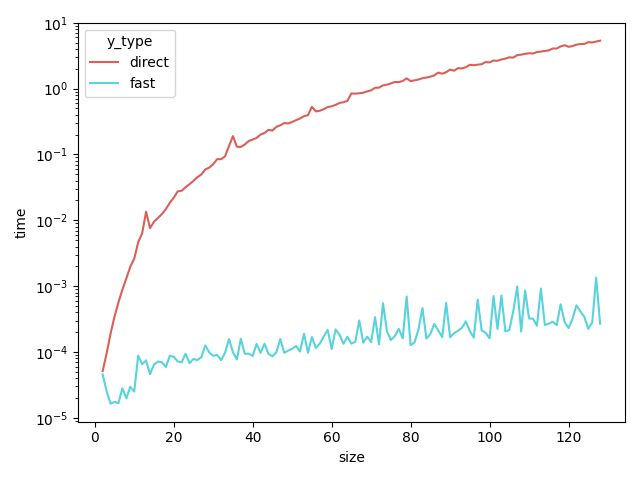
\includegraphics[width=0.8\textwidth]{../test/benchmark-results/bench-incremental-0.png}
  \caption{Confronto tra DCT diretta e veloce, sull'asse delle ascisse la
    dimensione delle metrici, sull'asse delle ordinate il tempo di esecuzione in
    scala logaritmica.}
  \label{fig:incremental-benchmark}
\end{figure}

Come si può osservare dal grafico in Figura
\ref{fig:incremental-benchmark}, il tempo computazione della DCT calcolata
tramite il metodo diretto cresce in maniera decisamente più rapida rispetto a
quello della DCT calcolata tramite la libreria \texttt{fft} di \texttt{scipy}.

La DCT calcolata tramite il metodo diretto presenta tempi proporzionali a $N^3$
rendendola quindi inutilizzabile per matrici di grandi dimensioni, la DCT calcolata
tramite la libreria \texttt{fft} di \texttt{scipy} invece presenta tempi di esecuzione 
decisamente migliori.

Siccome la libreria \texttt{fft} di \texttt{scipy} utilizza la FFT, si è scelto
di mettere a confronto i tempi di esecuzione della traformatata DCT2 su input di
dimensioni pari a potenze di 2 crescenti.

\begin{figure}[H]
  \centering
  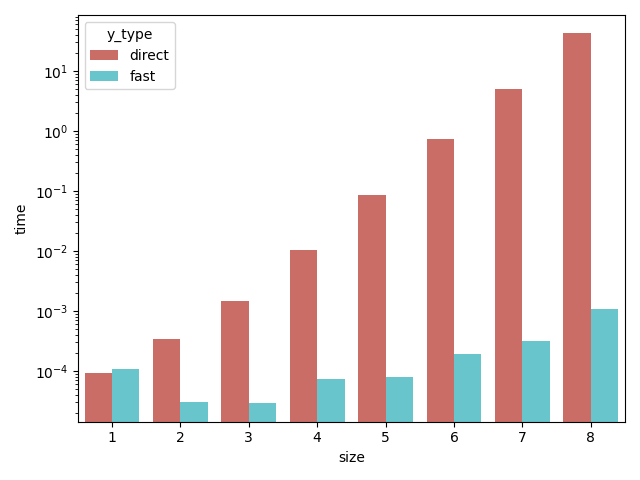
\includegraphics[width=0.8\textwidth]{../test/benchmark-results/bench-order-0.png}
  \caption{Confronto tra DCT diretta e veloce su input di dimensione pari a
    potenze di 2. Sull'asse delle ordinate il tempo in scala logaritmica,
    sull'asse delle ascisse le potenze di due delle dimensioni delle matrici.}
  \label{fig:order-benchmark}
\end{figure}

Anche in questo caso, come si può osservare dal grafico in
\ref{fig:order-benchmark}, la DCT implementata tramite il medoto diretto risulta
considerevolmente più lenta rispetto a quella implementata tramite la libreria
\texttt{fft} di \texttt{scipy}.


\section{Compressione di immagini}
La seconda parte della consegna richiede la realizzazione di un'interfaccia
grafica che permetta di caricare un'immagine in formato \texttt{BMP} in toni di
grigio e di applicare un algoritmo di compressione JPEG senza però utilizzare una
matrice di quantizzazione.

Anche per la realizzazione di questa seconda parte si è scelto di utilizzare
Python, in particolare, l'interfaccia grafica è stata realizzata tramite la
libreria \texttt{tkinter}.

Il software implementato permette all'utente di caricare un immagine
\texttt{BMP} in scala di grigi dal proprio filesystem sfruttando il \textit{file
  picker} di \texttt{tkinter}.

Una volta caricata l'immagine all'interno dell'applicazione, l'utente è in grado
di specificare:

\begin{itemize}
  \item un intero $F$ corrispondente alla dimensione in pixel dei
        \textit{macro-blocchi} su cui effettuare la DCT2.
  \item un intero $d$ compreso tra $0$ e $2F - 2$ rappresentante il valore di
        taglio delle frequenza
\end{itemize}

Una volta trasfrormata l'immagine, l'applicazione mostra fianco a fianco
l'immagine originale e quella su cui è stato eseguito l'algoritmo di
compressione delle frequenze. L'applicazione permette inoltre lo zoom e il pan
delle due immagini simultaneamente.

\textsc{AGGIUNGERE SCREENSHOT APPLICAZIONI}


\end{document}
